\documentclass[a4paper, 11pt]{article}
\usepackage{geometry}
\geometry{letterpaper, margin=1in}
\usepackage{amsmath}
\usepackage{amssymb}  
\usepackage{amsthm}
\usepackage{ulem} 
\usepackage{graphicx}
\usepackage{cancel} 
\usepackage{enumitem} 
\graphicspath{ {images/} }


\newtheorem*{theorem}{Theorem}
\newtheorem*{corollary}{Corollary}
\newtheorem*{lemma}{Lemma}
\newtheorem*{definition}{Definition}

\begin{document}
	%Header-Make sure you update this information!!!!
	\noindent
	\large\textbf{Thermal Physics - PH441} \hfill \textbf{John Waczak} \\
	\normalsize Day 25 \hfill  Date: \today \\
	
\subsection*{Thermo Review} 
	Quick review 
		\begin{align*}
			Q &= \int T dS \\ 
			W = - \int p dV \\ 
			\Delta U &= Q + W 
		\end{align*}

\subsection*{Ideal Gas Review} 
	\begin{align*}
		pV &= NkT \\ 
		U &= \frac{3}{2}NkT \\ 
		S &= Nk\Big(\ln\Big(\frac{n_Q}{n}\Big)+\frac{5}{2}\Big) \\ 
		F &= NkT\Big(\ln\Big(\frac{n}{n_Q}\Big)-1\Big) \\ 
		n &= n_Qe^{-\beta \mu} \\ 
		n_Q &= \Big(\frac{mkT}{2\pi \hbar^2}\Big)^{3/2} \\ 
	\end{align*}
	
\subsection*{Carnot Cycle} 
	What is a Carnot Cycle? It is a cycle with 4 steps. Start at $T_C$ the cold temperature. 
		\begin{enumerate}
			\item	Adiabatically (No Heat added) Compress until it is $T_H$ 
			\item 	Isothermally (fixed T) expand  (twice the volume) 
			\item 	Adiabatically expand to $T_C$ 
			\item 	Isothermally compress to original volume 
		\end{enumerate}
		\begin{figure}[!hbt]
			\centering
			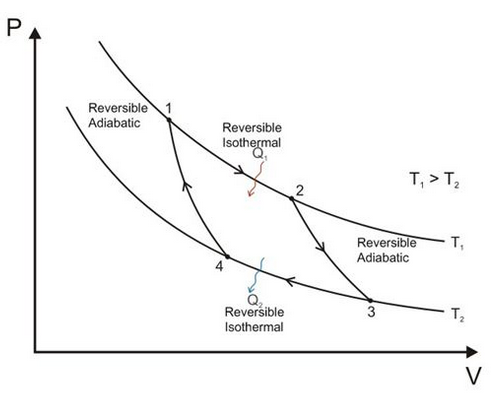
\includegraphics[width=0.65\columnwidth]{carnot}
		\end{figure}
		
	\begin{align*}
		Q_1 &= 0 \Rightarrow W_1 = \Delta U_1 \\ 
			&= \frac{3}{2}Nk(T_H-T_C) \\ 
		Q_3 &= 0 \Rightarrow W_3 = \frac{3}{2}Nk(T_C-T_H) \\ 
		Q_2 &= ?\\ 
		W_2 &\Rightarrow V_0\to 2_V)=0 \\ 
		W_2 &= -\int_{V_0}^{2V_0} \frac{1}{V}NkT_H \\ 
			&= -NkT_H\ln(2) \\ 
		S_{V_0} &= S_{V_4} \text{ and } S_{V_3} = S_{2V_0} \\ 
		\Rightarrow V4 &= \frac{1}{2} V_3 \text{ from entropy equation} \\ 
		\Rightarrow W_4 &= -NkT_C\ln(1/2)= NkT_C\ln(2) \\ 
		W_{TOT} &= k\ln(2)\cdot(T_C-T_H)
	\end{align*}
		
		
		
		
		
		
		
		
		
		
		
\end{document}


































